\section{RAR-XL: Clean full training: 2,500
steps}\label{record-docs-watermarking-qualitative-image-rar-weight-clean-full-2500-md-rar-xl-clean-full-training-2500-steps}

Candidate images are generated by modified weights using the same
requested class/index/seed. They can be different valid samples.

Eight pairs use fixed original indices 0, 64, 128, 192, 256, 320, 384
and 448. No detection or visual-quality filtering is applied.

\begin{recordfigure}
\centering
\pandocbounded{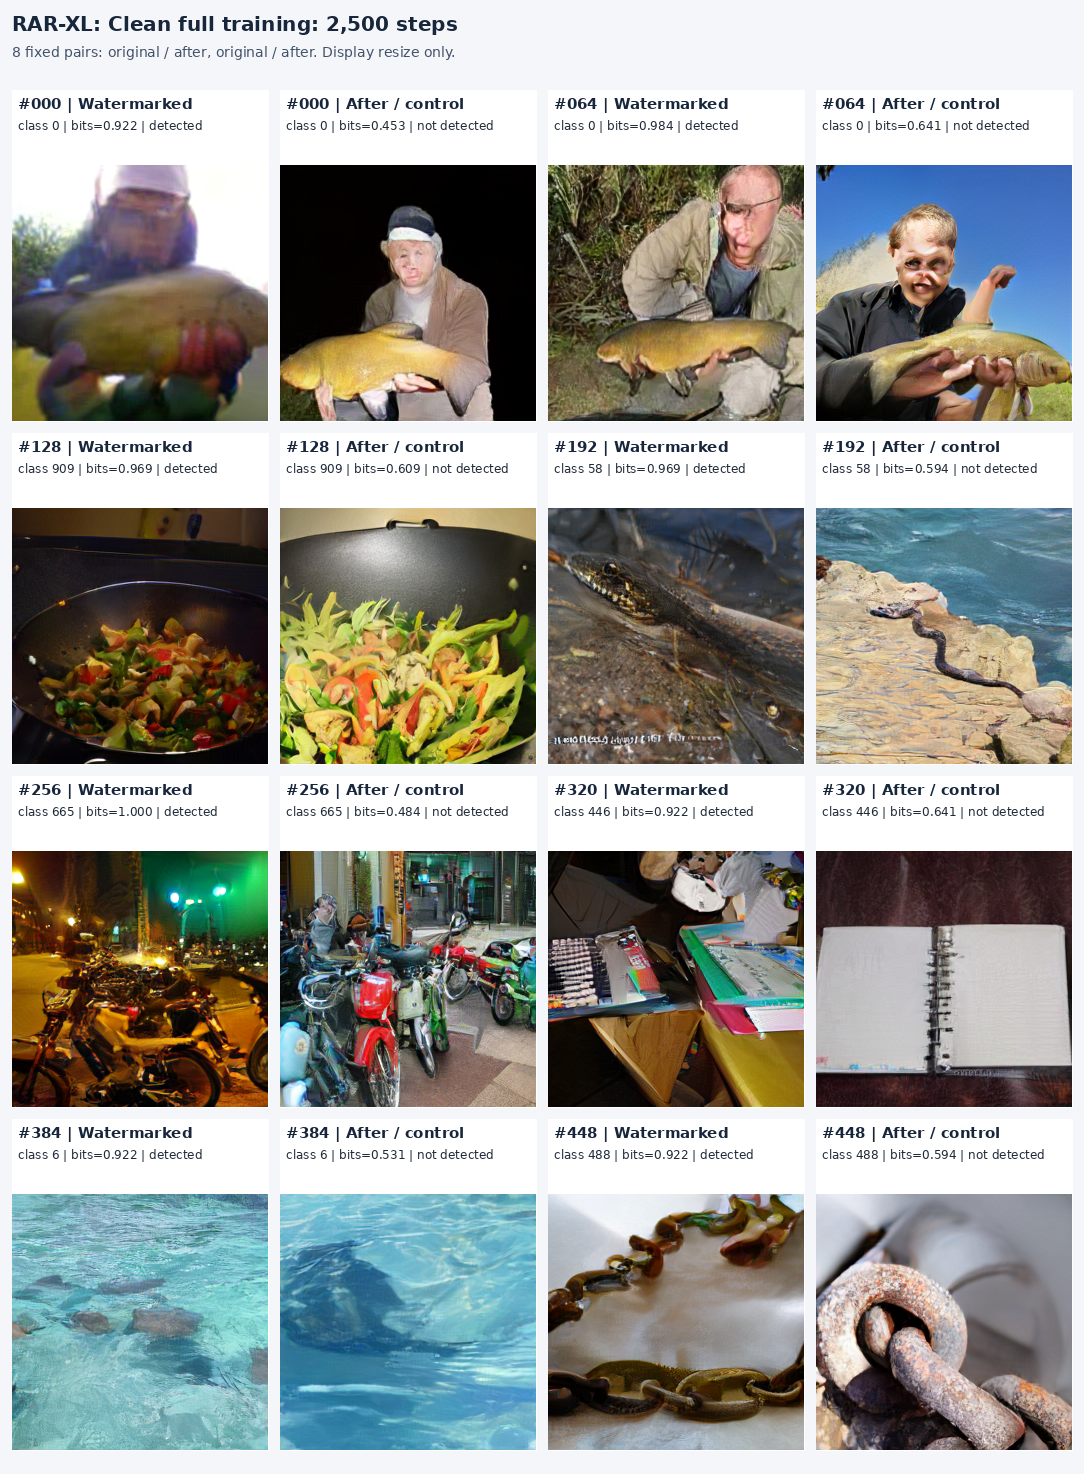
\includegraphics[keepaspectratio,alt={Eight original/after image pairs}]{figures/image-rar-weight-clean-full-2500.png}}
\caption{Eight original/after image pairs}
\end{recordfigure}

The lossless figure contains 16 panels. Each panel is displayed at 256
pixels; metrics use original native-resolution PNGs. Labels report each
output's detector result, not guaranteed removal.

{\scriptsize\setlength{\tabcolsep}{3pt}\def\LTcaptype{none} % do not increment counter
\begin{longtable}[]{@{}
  >{\raggedright\arraybackslash}p{(\linewidth - 10\tabcolsep) * \real{0.1667}}
  >{\raggedright\arraybackslash}p{(\linewidth - 10\tabcolsep) * \real{0.1667}}
  >{\raggedright\arraybackslash}p{(\linewidth - 10\tabcolsep) * \real{0.1667}}
  >{\raggedright\arraybackslash}p{(\linewidth - 10\tabcolsep) * \real{0.1667}}
  >{\raggedright\arraybackslash}p{(\linewidth - 10\tabcolsep) * \real{0.1667}}
  >{\raggedright\arraybackslash}p{(\linewidth - 10\tabcolsep) * \real{0.1667}}@{}}
\toprule\noalign{}
\begin{minipage}[b]{\linewidth}\raggedright
Index
\end{minipage} & \begin{minipage}[b]{\linewidth}\raggedright
Class
\end{minipage} & \begin{minipage}[b]{\linewidth}\raggedright
Before
\end{minipage} & \begin{minipage}[b]{\linewidth}\raggedright
After
\end{minipage} & \begin{minipage}[b]{\linewidth}\raggedright
LPIPS
\end{minipage} & \begin{minipage}[b]{\linewidth}\raggedright
Class CLIP
\end{minipage} \\
\midrule\noalign{}
\endhead
\bottomrule\noalign{}
\endlastfoot
0 & 0 & class 0 \textbar{} bits=0.922 \textbar{} detected & class 0
\textbar{} bits=0.453 \textbar{} not detected & 0.7932 & 0.3293 \\
64 & 0 & class 0 \textbar{} bits=0.984 \textbar{} detected & class 0
\textbar{} bits=0.641 \textbar{} not detected & 0.6747 & 0.3236 \\
128 & 909 & class 909 \textbar{} bits=0.969 \textbar{} detected & class
909 \textbar{} bits=0.609 \textbar{} not detected & 0.5895 & 0.3027 \\
192 & 58 & class 58 \textbar{} bits=0.969 \textbar{} detected & class 58
\textbar{} bits=0.594 \textbar{} not detected & 0.6060 & 0.3107 \\
256 & 665 & class 665 \textbar{} bits=1.000 \textbar{} detected & class
665 \textbar{} bits=0.484 \textbar{} not detected & 0.6478 & 0.2892 \\
320 & 446 & class 446 \textbar{} bits=0.922 \textbar{} detected & class
446 \textbar{} bits=0.641 \textbar{} not detected & 0.7911 & 0.2957 \\
384 & 6 & class 6 \textbar{} bits=0.922 \textbar{} detected & class 6
\textbar{} bits=0.531 \textbar{} not detected & 0.5538 & 0.2688 \\
448 & 488 & class 488 \textbar{} bits=0.922 \textbar{} detected & class
488 \textbar{} bits=0.594 \textbar{} not detected & 0.7062 & 0.2748 \\
\end{longtable}
}

\href{records/docs/watermarking/images.tex}{Image metrics} \textbar{}
\href{../docs/watermarking/README.md}{Report overview}
